\subsection{Urban Data Layer (UDL) - Administrative Boundaries Identification}
{{\footnotesize
\noindent UrbanDataLayer standardizes heterogeneous urban data formats and provides pipelines for tasks like air quality prediction and land-use classification, enabling the rapid creation of multi-modal urban benchmarks .


\begin{description}[labelwidth=4cm, labelsep=1em, leftmargin=4cm, itemsep=0.1em, parsep=0em]
  \item[date:] 2024-12-13
  \item[version:] v1.0
  \item[last\_updated:] 2024-12
  \item[expired:] unknown
  \item[valid:] yes
  \item[valid\_date:] 2024-12-13
  \item[url:] \href{https://neurips.cc/virtual/2024/poster/97837}{https://neurips.cc/virtual/2024/poster/97837}
  \item[doi:] unknown
  \item[domain:]
    - Climate \& Earth Science
  \item[focus:] Unified data pipeline for multi-modal urban science research
  \item[keywords:]
    - data pipeline
    - urban science
    - multi-modal
    - benchmark
  \item[licensing:] unknown
  \item[task\_types:]
    - Prediction
    - Classification
  \item[ai\_capability\_measured:]
    - Multi-modal urban inference
    - standardization
  \item[metrics:]
    - Task-specific accuracy or RMSE
  \item[models:]
    - Baseline regression/classification pipelines
  \item[ml\_motif:]
    - Classification
  \item[type:] Framework
  \item[ml\_task:]
    - Prediction, classification
  \item[solutions:] 0
  \item[notes:] Source code available on GitHub (SJTU-CILAB/udl); promotes reusable urban-science foundation models .

  \item[contact.name:] Yiheng Wang
  \item[contact.email:] unknown
  \item[results.links.name:] ChatGPT LLM
  \item[fair.reproducible:] Yes
  \item[fair.benchmark\_ready:] Yes
  \item[id:] urban\_data\_layer\_udl\_-\_administrative\_boundaries\_identification
  \item[Citations:] \cite{neurips2024_0db7f135}
\end{description}

{\bf Ratings:} ~ \\

\begin{tabular}{p{0.15\textwidth} p{0.07\textwidth} p{0.7\textwidth}}
\hline
Rating & Value & Reason \\
\hline
dataset & 5 & Large, multi-modal urban datasets are open-source, well-documented, and support
reproducible research.
 \\
documentation & 5 & GitHub repository and conference poster provide comprehensive code and reproducibility
instructions.
 \\
metrics & 5 & Uses task-specific accuracy and RMSE metrics appropriate for prediction and classification.
 \\
reference\_solution & 4 & Baseline models available but not exhaustive; community adoption and extensions expected.
 \\
software & 3 & Source code is publicly available on GitHub; baseline regression and classification
pipelines are included but framework maturity is moderate.
 \\
specification & 5 & Multiple urban science tasks like prediction and classification are well specified
with clear input/output and evaluation criteria.
 \\
\hline
\end{tabular}

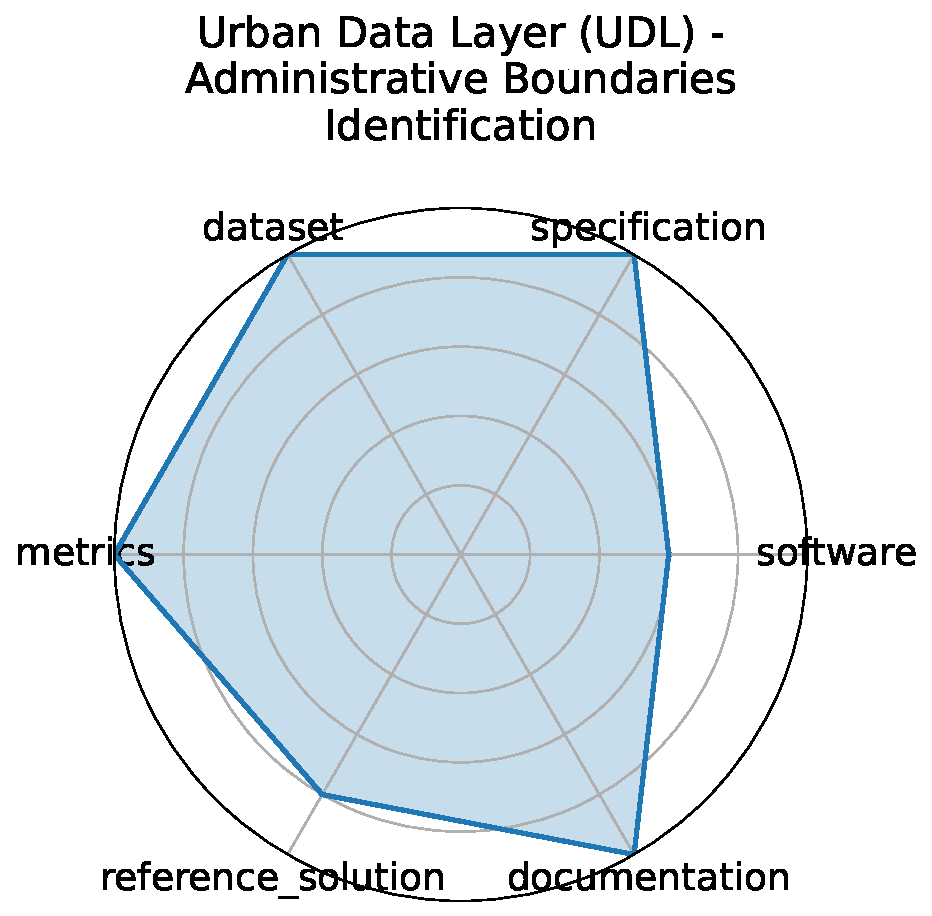
\includegraphics[width=0.2\textwidth]{urban_data_layer_udl_-_administrative_boundaries_identification_radar.pdf}
}}
\clearpage